\documentclass[a4paper]{article}

\usepackage[english]{babel}
\usepackage[utf8]{inputenc}
\usepackage{amsmath}
\usepackage{graphicx}
\usepackage[colorinlistoftodos]{todonotes}
\usepackage{hyperref}

\title{Capstone Project for Udacity Machine Learning Nanodegree}

\author{Pär Steffansson}

\date{\today}

\begin{document}
\maketitle

\begin{abstract}
I selected the competition \href{https://www.kaggle.com/c/zillow-prize-1#description}{Zillow Prize} found at
\href{https://www.kaggle.com}{Kaggle} as the Capstone project in my \textit{Machine Learning Engineer Nanodegree}
provided by \href{https://www.udacity.com}{Udacity}.
\end{abstract}

\tableofcontents

\section{Project Definition}
An overview of the project definition is described below. For more details see the competition
\href{https://www.kaggle.com/c/zillow-prize-1#description}{Zillow Prize}.

\subsection{Project Overview}
%
% Student provides a high-level overview of the project in layman’s terms. Background information such as the
% problem domain, the project origin, and related data sets or input data is given.
%
I selected the competition \href{https://www.kaggle.com/c/zillow-prize-1#description}{Zillow Prize} found at
\href{https://www.kaggle.com}{Kaggle} as the Capstone project in my \textit{Machine Learning Engineer Nanodegree}
provided by \href{https://www.udacity.com}{Udacity}.

\href{https://www.zillow.com}{Zillow} is the leading real estate and rental marketplace dedicated to empowering
consumers with data. They launched the Kaggle competition \textit{Zillow Prize} to improve their ability to predict
house prices.

I selected this competition to learn from the rich source of knowledge the community around these competitions
provide. Comparing and learning from public Kernels provided gives a good benchmark of cutting edge models
for these kind of problems.

\subsection{Problem Statement}
%
% The problem which needs to be solved is clearly defined. A strategy for solving the problem, including discussion
% of the expected solution, has been made.
%
They have been developing their own model to predict prices for years. The problem at hand is to see if the
Kaggle community can improve on it creating an even better model.

\subsection{Metrics}
%
% Metrics used to measure performance of a model or result are clearly defined. Metrics are justified based on the
% characteristics of the problem.
%
The metric is defined by Zillow witch is asking to predict the \textit{logerror} between their Zestimate model and the
actual sale price, given all the features of a home. The log error is defined as
\[ logerror = log(Zestimate) - log(SalePrice) \]


\section{Analysis}

\subsection{Data Exploration}
% If a dataset is present, features and calculated statistics relevant to the problem have been reported and
% discussed, along with a sampling of the data. In lieu of a dataset, a thorough description of the input space or
% input data has been made. Abnormalities or characteristics about the data or input that need to be addressed
% have been identified.
This data exploration is inspired by the [Simple Exploration Notebook - Zillow Prize](https://www.kaggle.com/sudalairajkumar/simple-exploration-notebook-zillow-prize)
written by Kaggle Grandmaster [SRK](https://www.kaggle.com/sudalairajkumar).

We will be working with following data files
\begin{itemize}
    \item \textit{properties\_2016.csv} - all the properties with their home features for 2016. Note: Some 2017 new
    properties don't have any data yet except for their parcelid's. Those data points should be populated when
    properties\_2017.csv is available.
    \item \textit{train\_2016.csv} - the training set with transactions from 1/1/2016 to 12/31/2016.
    \item \textit{sample\_submission.csv} - a sample submission file in the correct format
\end{itemize}

\subsubsection{Traning Set File}
The training set in file \textit{train\_2016.csv} contains 90275 rows and three columns
\begin{itemize}
    \item \textit{parcelid} - which is the id of the property.
    \item \textit{logerror} - the log-error comparing the log of the actual price and the log of the predicted price.
    \item \textit{transactiondate} - is the date when the property was sold
\end{itemize}

Each row correspond to a property transaction and there will be more than one row in this file with the same
parcelid if the property has been sold more than ones during 2016. In fact counting there are
\begin{itemize}
    \item 90026 properties that have been sold ones
    \item 123 properties that have been sold twice
    \item and one property that was sold one time.
\end{itemize}

\begin{figure}
\centering
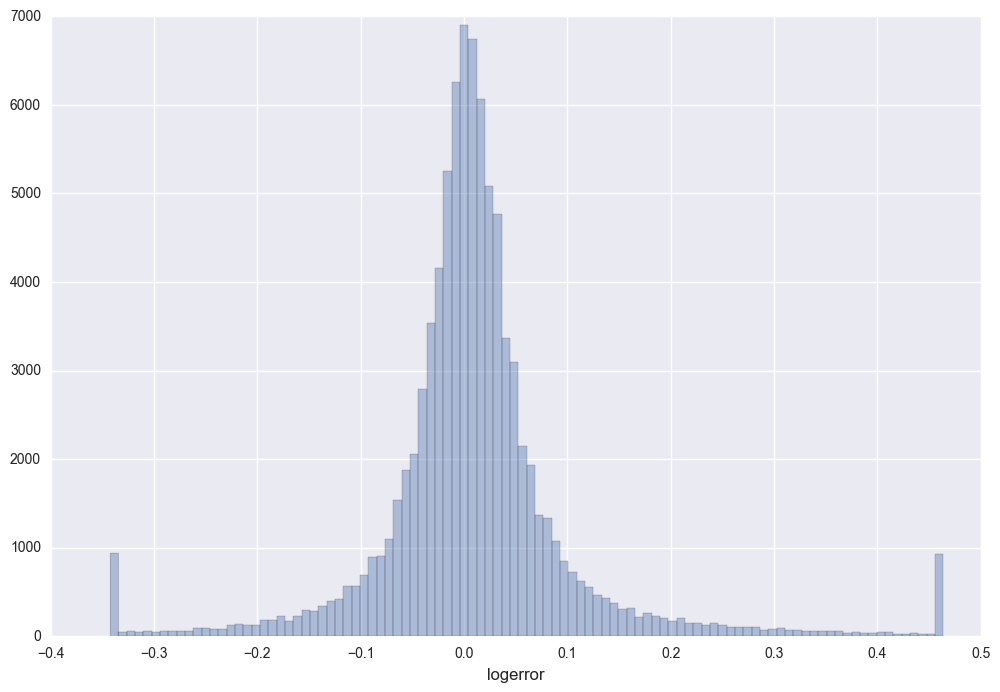
\includegraphics[width=1\textwidth]{./img/train-logerror.png}
\caption{\label{fig:logerror}Logerror distribution}
\end{figure}
Looking at Figure \ref{fig:logerror} the log error has nice normal distribution centered around zero.

\begin{figure}
\centering
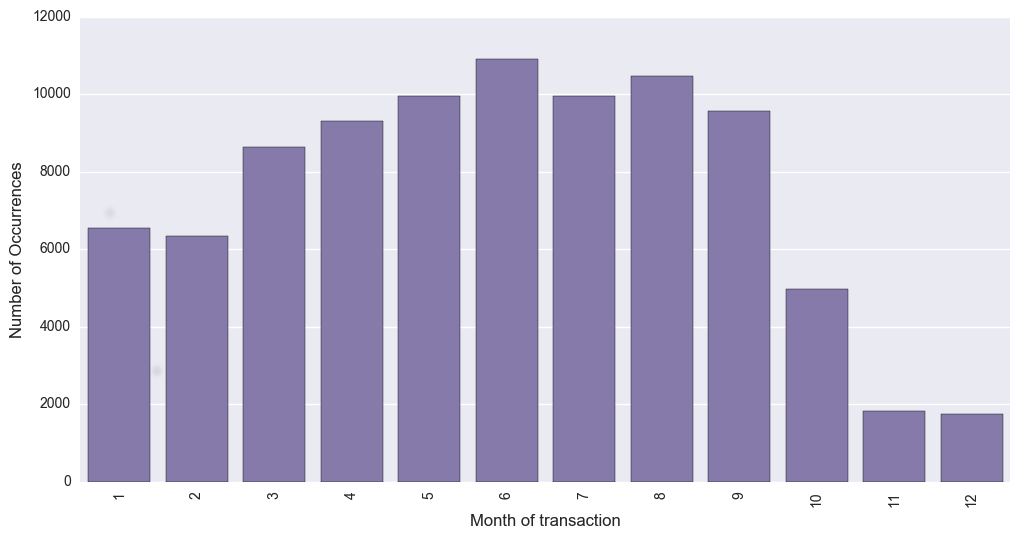
\includegraphics[width=1\textwidth]{./img/train-transactiondate.png}
\caption{\label{fig:transactions}Number of transactions over time}
\end{figure}
According to Zillow the training data has all the transactions before October 15, 2016, plus some of the transactions
after October 15, 2016. Looking at Figure \ref{fig:transactions} from January to September there are about 6000-11000
transactions per month while dropping to under 2000 in November to December.

\subsubsection{Properties}
Property data file \textit{properties\_2016.csv} is a lat larger with 2985217 rows and 58 columns describing home
features. The file seems like some of the columns contain less information in the form of NaN values. Lets us look at
that more closely.
![](./prop-nan.png)
Just looking at the data visually more than half of the data is not there and the data loss is unevenly distributed
on the featues. Even if we have a lot of features about 30 percent will most likely not contribute to a better
model when they do not contain any information.


%Exploratory Visualization
%A visualization has been provided that summarizes or extracts a relevant characteristic or feature about the dataset
%or input data with thorough discussion. Visual cues are clearly defined.

\subsection{Algorithms and Techniques}
% Algorithms and techniques used in the project are thoroughly discussed and properly justified based on
% the characteristics of the problem.

\subsection{Benchmark}
% Student clearly defines a benchmark result or threshold for comparing performances of solutions obtained.

\section{Methodology}

\subsection{Data Preprocessing}
% All preprocessing steps have been clearly documented. Abnormalities or characteristics about the data or
% input that needed to be addressed have been corrected. If no data preprocessing is necessary, it has been
% clearly justified.

\subsection{Implementation}
% The process for which metrics, algorithms, and techniques were implemented with the given datasets or input
% data has been thoroughly documented. Complications that occurred during the coding process are discussed.
```

\subsection{Refinement}
% The process of improving upon the algorithms and techniques used is clearly documented. Both the initial and
% final solutions are reported, along with intermediate solutions, if necessary.

\section{Results}

\subsection{Model Evaluation and Validation}
% The final model’s qualities — such as parameters — are evaluated in detail. Some type of analysis is used
% to validate the robustness of the model’s solution.

\subsection{Justification}
% The final results are compared to the benchmark result or threshold with some type of statistical analysis.
% Justification is made as to whether the final model and solution is significant enough to have adequately
% solved the problem.

\section{Conclusion}

\subsection{Free-Form Visualization}
% A visualization has been provided that emphasizes an important quality about the project with thorough discussion.
% Visual cues are clearly defined.

\subsection{Reflection}
% Student adequately summarizes the end-to-end problem solution and discusses one or two particular aspects of
% the project they found interesting or difficult.

\subsection{Improvement}
% Discussion is made as to how one aspect of the implementation could be improved. Potential solutions resulting
% from these improvements are considered and compared/contrasted to the current solution.




%%%%%%%%%%%%% remove all below


\section{Introduction 5 lines to max 1/2 page}
\label{sec:introduction}

Explain the context of the experiment here. Why is condensed matter physics interesting or important?
Optional things you could talk about (but don't have to -- this is up to you): transistors, computers, Quantum computers, fundamental knowledge (e.g. the resistance quantum).

Briefly explain what methods you will use in the experiment, and what values you will extract from the data.

For this section and all following sections: If you refer to an equation, previous result or theory that is not regarded as common knowledge, then cite the source (article or book) where you found this. For example, you can cite the Nano 3 Lecture notes \cite{nano3}.

\section{Theory 2-3 pages}
\label{sec:theory}

\subsection{Two-dimensional Electron Gas}
Here, explain the concept of a 2-DEG in GaAs/AlGaAs. What is a 2-DEG and why does it arise?

\subsection{Hall Effect}
Explain the classical Hall effect in your own words. What do I measure at $B=0$? And what happens if $B>0$? Which effect gives rise to the voltage drop in the vertical direction?

\subsection{Quantum Hall Effect}
Explain the IQHE in your own words. What does the density of states look like in a 2-DEG when $B=0$? What are Landau levels and how do they arise? What are edge states? What does the electron transport look like when you change the magnetic field? What do you expect to measure?

\section{Experiment 1-2 pages}
\subsection{Fabrication}
Explain a step-by-step recipe for fabrication here. How long did you etch and why? What is an Ohmic contact?
\subsection{Experimental set-up}
Explain the experimental set-up here. Use a schematic picture (make it yourself in photoshop, paint, ...) to show how the components are connected. Briefly explain how a lock-in amplifier works.

\section{Results and interpretation 2-3 pages}
Show a graph of the longitudinal resistivity ($\rho_{xx}$) and Hall resistivity ($\rho_{xy}$) versus magnetic field, extracted from the raw data shown in figure \ref{fig:data}. You will have the link to the data in your absalon messages, if not e-mail Guen (guen@nbi.dk). Explain how you calculated these values, and refer to the theory.

\begin{figure}
\centering
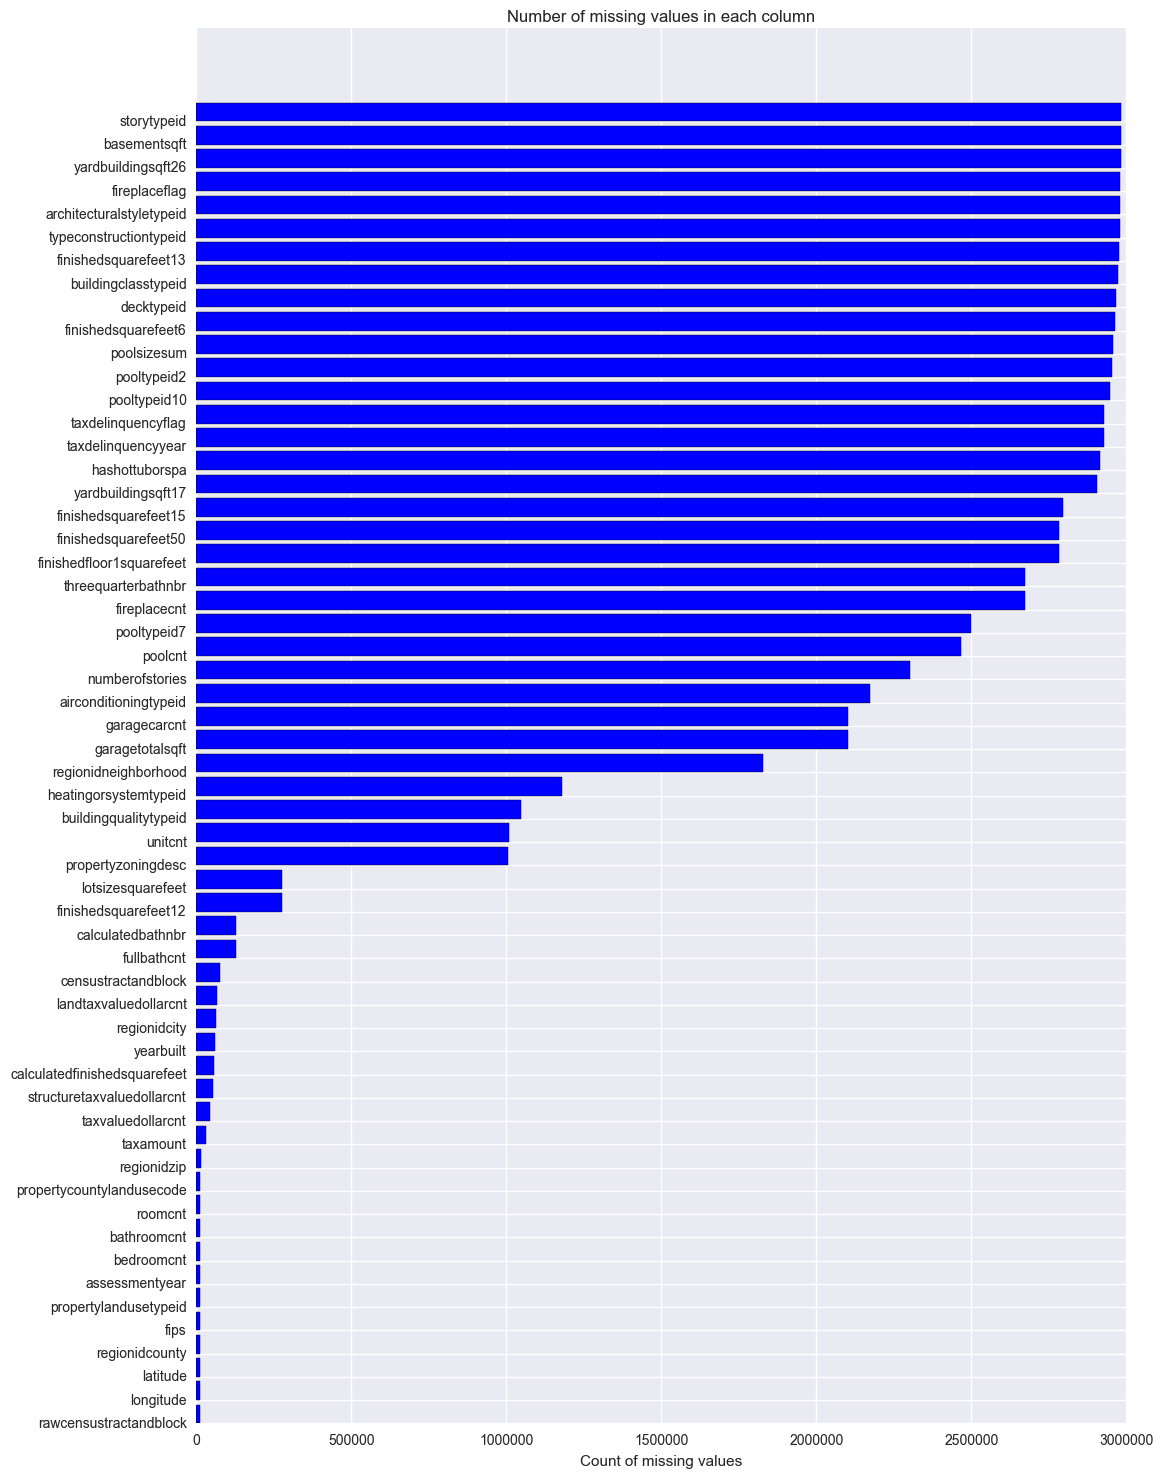
\includegraphics[width=1\textwidth]{./img/prop-nan.png}
\caption{\label{fig:data}Raw (unprocessed) data. Replace this figure with the one you've made, that shows the resistivity.}
\end{figure}

\subsection{Classical regime}
Calculate the sheet electron density $n_{s}$ and electron mobility $\mu$ from the data in the low-field regime, and refer to the theory in section \ref{sec:theory}. Explain how you retrieved the values from the data (did you use a linear fit?).
Round values off to 1 or 2 significant digits: 8.1643 ~= 8.2. Also, 5e-6 is easier to read than 0.000005.

!OBS: This part is optional (only if you have time left).
Calculate the uncertainty as follows: \newline $u(f(x, y, z)) = \sqrt{(\frac{\delta f}{\delta{x}} u(x))^{2} + (\frac{\delta f}{\delta{y}} u(y))^{2} + (\frac{\delta f}{\delta{z}} u(z))^{2}}$, where $f$ is the calculated value ($n_{s}$ or $\mu$), $x, y, z$ are the variables taken from the measurement and $u(x)$ is the uncertainty in x (and so on).

\subsection{Quantum regime}
Calculate $n_{s}$ for the high-field regime.
Show a graph of the longitudinal conductivity ($\rho_{xx}$) and Hall conductivity($\rho_{xy}$) \textbf{in units of the resistance quantum} ($\frac{h}{e^{2}}$), depicting the integer filling factors for each plateau.
Show a graph of the plateau number versus its corresponding value of $1/B$. From this you can determine the slope, which you use to calculate the electron density.
Again, calculate the uncertainty for your obtained values.

\section{Discussion 1/2-1 page}
Discuss your results. Compare the two values of $n_{s}$ that you've found in the previous section. Compare your results with literature and comment on the difference. If you didn't know the value of the resistance quantum, would you be able to deduce it from your measurements? If yes/no, why?

\newpage
\section{Some LaTeX tips}
\label{sec:latex}
\subsection{How to Include Figures}

First you have to upload the image file (JPEG, PNG or PDF) from your computer to writeLaTeX using the upload link the project menu. Then use the includegraphics command to include it in your document. Use the figure environment and the caption command to add a number and a caption to your figure. See the code for Figure \ref{fig:frog} in this section for an example.

\begin{figure}
\centering
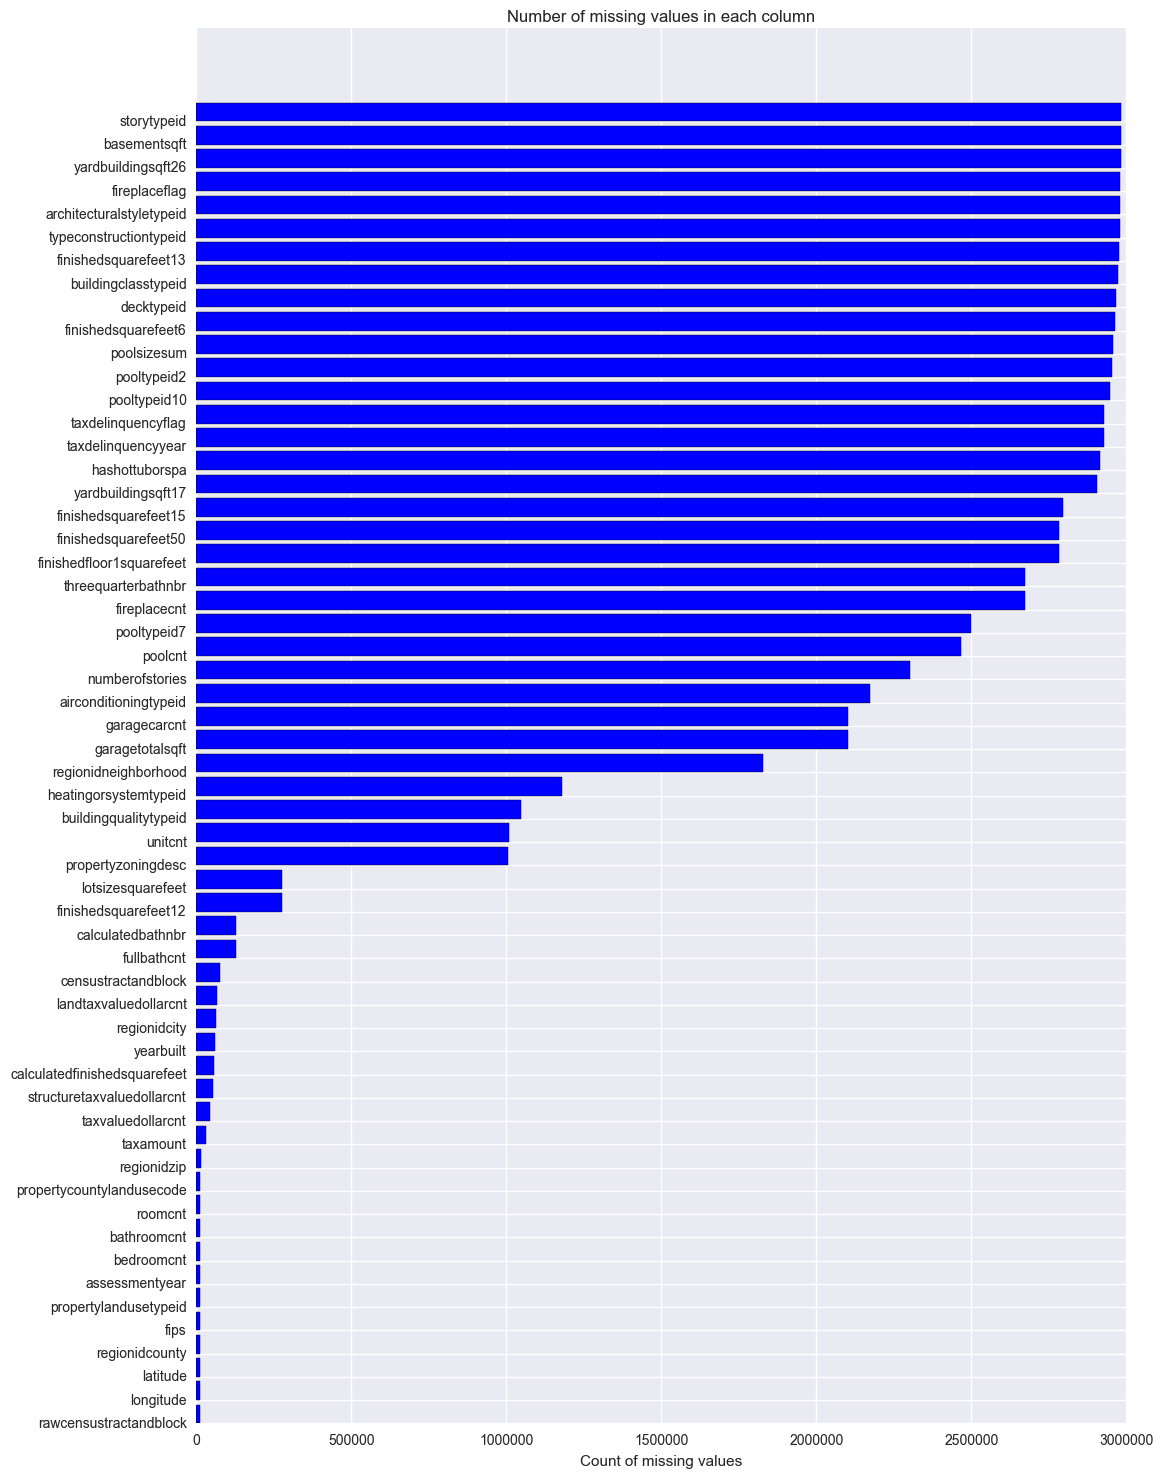
\includegraphics[width=0.3\textwidth]{./img/prop-nan.png}
\caption{\label{fig:frog}This frog was uploaded to writeLaTeX via the project menu.}
\end{figure}

\subsection{How to Make Tables}

Use the table and tabular commands for basic tables --- see Table~\ref{tab:widgets}, for example.

\begin{table}
\centering
\begin{tabular}{l|r}
Item & Quantity \\\hline
Widgets & 42 \\
Gadgets & 13
\end{tabular}
\caption{\label{tab:widgets}An example table.}
\end{table}

\subsection{How to Write Mathematics}

\LaTeX{} is great at typesetting mathematics. Let $X_1, X_2, \ldots, X_n$ be a sequence of independent and identically distributed random variables with $\text{E}[X_i] = \mu$ and $\text{Var}[X_i] = \sigma^2 < \infty$, and let

\begin{equation}
S_n = \frac{X_1 + X_2 + \cdots + X_n}{n}
      = \frac{1}{n}\sum_{i}^{n} X_i
\label{eq:sn}
\end{equation}

denote their mean. Then as $n$ approaches infinity, the random variables $\sqrt{n}(S_n - \mu)$ converge in distribution to a normal $\mathcal{N}(0, \sigma^2)$.

The equation \ref{eq:sn} is very nice.

\subsection{How to Make Sections and Subsections}

Use section and subsection commands to organize your document. \LaTeX{} handles all the formatting and numbering automatically. Use ref and label commands for cross-references.

\subsection{How to Make Lists}

You can make lists with automatic numbering \dots

\begin{enumerate}
\item Like this,
\item and like this.
\end{enumerate}
\dots or bullet points \dots
\begin{itemize}
\item Like this,
\item and like this.
\end{itemize}
\dots or with words and descriptions \dots
\begin{description}
\item[Word] Definition
\item[Concept] Explanation
\item[Idea] Text
\end{description}

We hope you find write\LaTeX\ useful, and please let us know if you have any feedback using the help menu above.

\begin{thebibliography}{9}
\bibitem{nano3}
  K. Grove-Rasmussen og Jesper Nygård,
  \emph{Kvantefænomener i Nanosystemer}.
  Niels Bohr Institute \& Nano-Science Center, Københavns Universitet

\end{thebibliography}
\end{document}